\chapter{الجريانات اللزجة}\label{ch:b2:viscous-flows}

أمِل وعاء عسل فينسكب شريطًا بطيئًا كثيفًا؛ وأمِل وعاء ماء
فيختفي. وحرّك ملعقة في كل منهما: فالعسل يقاوم، ويظل يقاوم عند
أي سرعة؛ وأما الماء فلا يكاد يبالي حتى تسرع، فيدوّم عندئذ.
والفرق هو \emph{\omterm{def:b2:viscous-flows:viscosity}{اللزوجة}} --- أي احتكاك المائع الداخلي --- والصراع
بين \omterm{def:b2:viscous-flows:viscosity}{اللزوجة} والعطالة، ملخَّصًا في عدد واحد هو \omterm{def:b2:viscous-flows:reynolds}{عدد رينولدز}، هو
الذي يقرّر أيزحف الجريان في طبقات منظَّمة أم يتقلّب اضطرابًا.
وهذا الفصل يضيف القوة اللزجة إلى \omterm{thm:b2:euler-bernoulli:euler}{معادلة أويلر}، ويحلّ
الجريانين الصفائحيين اللذين يستعملهما كل مهندس، ويشرح لماذا
تختبئ \omterm{def:b2:viscous-flows:viscosity}{اللزوجة}، عند \omterm{def:b2:viscous-flows:reynolds}{عدد رينولدز} الكبير، في طبقة رقيقة عند
الجدار ومع ذلك تكلّف كل سيارة وسفينة وطائرة معظم وقودها.

\begin{omfigure}
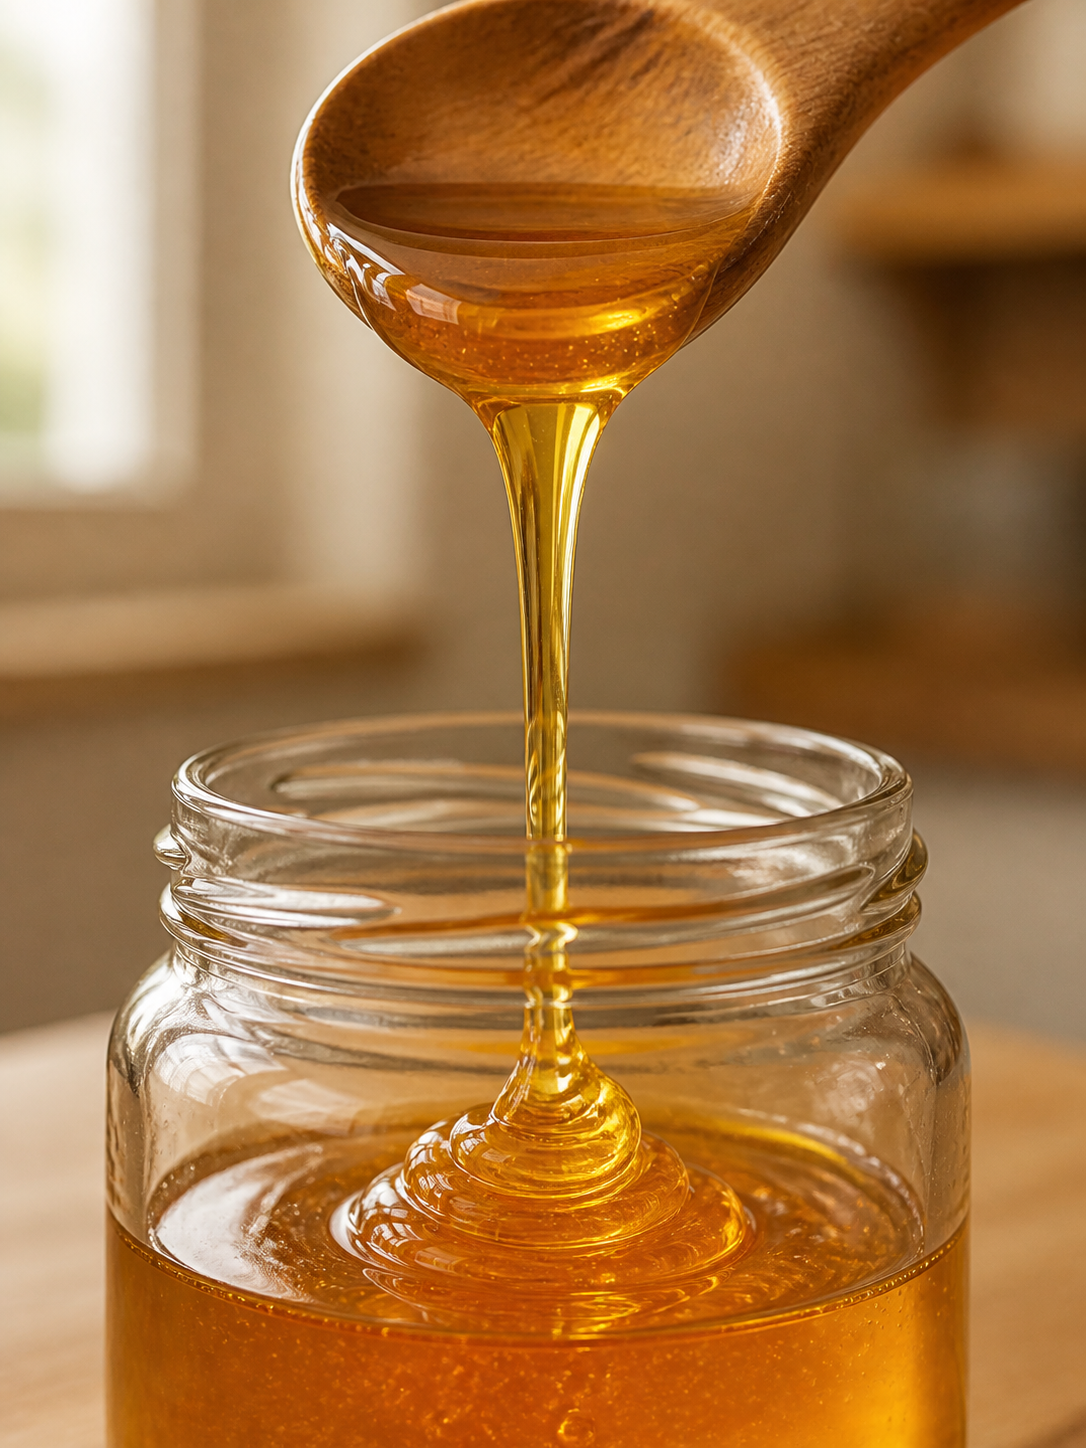
\includegraphics[width=0.34\linewidth]{images/book4/ai/b4-04-honey-spoon-viscous.png}

{\small ينسكب العسل شريطًا رفيعًا مستقرًّا يلتفّ حين يهبط: \omterm{def:b2:viscous-flows:viscosity}{لزوجة} تفوق \omterm{def:b2:viscous-flows:viscosity}{لزوجة} الماء عشرة آلاف مرة تجعل العطالة عديمة الشأن --- أي جريانًا زاحفًا.}
\end{omfigure}


\section{اللزوجة ومعادلة نافييه--ستوكس}

\begin{definition}[اللزوجة النيوتنية]\label{def:b2:viscous-flows:viscosity}
\index{لزوجة}\index{لزوجة ديناميكية}\index{لزوجة حركية}\index{إجهاد القصّ}\index{مائع نيوتني}
في جريان قصّ مستو $\vect v = v_x(y)\,\vect e_x$، يؤثر المائع فوق سطح
$y = \text{ثابت}$ في المائع تحته (عبر عنصر
سطحي $\dd S$) بالقوة المماسية
\[
\dd\vect F = \eta\,\frac{\dd v_x}{\dd y}\,\dd S\;\vect e_x ,
\]
فيجرّ الطبقةَ الأبطأ إلى الأمام ويُجرّ إلى الخلف في المقابل.
و\emph{إجهاد القصّ} هو $\tau = \eta\,\dd v_x/\dd y$؛ والمعامل
$\eta$ (ووحدته \unit{Pa.s}) هو \emph{اللزوجة الديناميكية} للمائع،
و $\nu = \eta/\rho$ (\unit{m^2/s}) هي \emph{لزوجته الحركية}. والمائع
الذي لا تتوقف $\eta$ فيه على معدل القصّ \emph{نيوتني}: كالماء
والهواء والزيوت والكحول؛ وأما الدم والطلاء ومعجون الطماطم
ومصاهر البوليمرات فليست كذلك. ورتب القدر عند \qty{20}{\degreeCelsius}: الهواء $\eta =
\qty{1.8e-5}{Pa.s}$ ($\nu = \qty{1.5e-5}{m^2/s}$)، والماء $\qty{1.0e-3}{Pa.s}$
($\nu = \qty{1.0e-6}{m^2/s}$)، وزيت الزيتون $\qty{0.08}{Pa.s}$، والغليسرول
$\qty{1.5}{Pa.s}$، والعسل $\sim\qty{10}{Pa.s}$. وتخفّ السوائل بالتسخين،
وتثقل الغازات.
\end{definition}

\begin{proposition}[كثافة القوة اللزجة؛ شرط اللاانزلاق]\label{prop:b2:viscous-flows:density}
\index{شرط اللاانزلاق}\index{كثافة القوة اللزجة}
في جريان القصّ المستوي، تكون القوة اللزجة الصافية على شريحة
مائع بين $y$ و $y + \dd y$، في واحدة الحجم، $\eta\,\dd^2v_x/\dd y^2$:
أي إن \omterm{def:b2:viscous-flows:viscosity}{اللزوجة} تؤثر ككثافة قوة حجمية $\eta\,\Delta\vect v$ (واللابلاسي
مأخوذ مركّبةً مركّبةً)، وهي نتيجة صحيحة في أي \omterm{cor:b2:fluid-kinematics:incompressible}{جريان
لاانضغاطي}. وعند جدار صلب \emph{يلتصق} المائع: فتساوي سرعته سرعة
الجدار (وهو \emph{\omterm{prop:b2:viscous-flows:density}{شرط اللاانزلاق}})، ولهذا يبقى الغبار على ريشة
مروحة ويحسّ الجدار إعاقة لزجة.
\end{proposition}

\begin{proof}
تُجذب الشريحة بالقوة $\eta\,v_x'(y + \dd y)\dd S$ من الأعلى وبالقوة
$-\eta\,v_x'(y)\dd S$ من الأسفل: فالصافي $\eta v_x''\,\dd y\,\dd S$. والصيغة
العامة مسلَّم بها (وهي تنتج من كتابة الإجهاد دالةً خطية
متناظرة في تدرجات السرعة). وأما \omterm{prop:b2:viscous-flows:density}{شرط اللاانزلاق} فتجريبي.
\end{proof}

\begin{theorem}[معادلة نافييه--ستوكس]\label{thm:b2:viscous-flows:ns}
\index{معادلة نافييه--ستوكس}
يحقق \omterm{def:b2:viscous-flows:viscosity}{مائع نيوتني} لاانضغاطي
\[
\rho\Bigl(\frac{\partial\vect v}{\partial t} + (\vect v\cdot\operatorname{\vect{grad}})
\vect v\Bigr) = -\operatorname{\vect{grad}}P + \rho\vect g + \eta\,\Delta\vect v ,
\qquad \operatorname{div}\vect v = 0 ,
\]
مع \omterm{prop:b2:viscous-flows:density}{شرط اللاانزلاق} على كل جدار. \omterm{thm:b2:euler-bernoulli:euler}{ومعادلة أويلر} هي الحالة
$\eta = 0$.
\end{theorem}
\admitted

\begin{omfigure}
\begin{tikzpicture}[font=\small, x=1cm, y=1cm, >=Stealth]
  \begin{scope}
    \draw[thick] (-0.2,0) -- (3.6,0); \fill[pattern=north east lines] (-0.2,-0.18) rectangle (3.6,0);
    \draw[thick, omExo] (-0.2,2.2) -- (3.6,2.2); \fill[pattern=north east lines, pattern color=omExo] (-0.2,2.2) rectangle (3.6,2.38);
    \draw[omExo, very thick, ->] (1.4,2.6) -- (2.6,2.6) node[right, font=\footnotesize] {$U$};
    \foreach \y in {0.4,0.8,...,2.0} \draw[omDef, thick, ->] (0.4,\y) -- ({0.4+1.1*\y/2.2*1.8},\y);
    \draw[omDef, thick] (0.4,0) -- (2.2,2.2);
    \node[font=\footnotesize] at (1.8,-0.5) {كويت: $v_x = Uy/h$، $\tau = \eta U/h$};
    \draw[<->] (3.3,0) -- (3.3,2.2) node[midway, right, font=\footnotesize] {$h$};
  \end{scope}
  \begin{scope}[xshift=7.2cm]
    \draw[thick, fill=omDef!10] (0,0.6) rectangle (3.0,1.6);
    \draw[omThm, very thick, ->] (1.5,1.6) -- (2.6,1.6) node[above, font=\footnotesize] {$\eta v_x'(y+\dd y)\,\dd S$};
    \draw[omThm, very thick, ->] (1.5,0.6) -- (0.4,0.6) node[below, font=\footnotesize] {$\eta v_x'(y)\,\dd S$};
    \node[font=\footnotesize] at (-0.5,1.6) {$y + \dd y$};
    \node[font=\footnotesize] at (-0.4,0.6) {$y$};
    \node[font=\footnotesize] at (1.5,-0.5) {الصافي: $\eta\,v_x''\,\dd y\,\dd S$};
  \end{scope}
\end{tikzpicture}

{\small على اليسار: جريان كويت المستوي بين صفيحة ثابتة وصفيحة
تتحرك بالسرعة $U$ --- منحني سرعات خطي، \omterm{def:b2:viscous-flows:viscosity}{وإجهاد القصّ} نفسه على كل
طبقة. وعلى اليمين: القوى اللزجة على شريحة مائع؛ وهي تتلاشى ما
لم يكن منحني السرعات محدَّبًا.}
\end{omfigure}

\begin{example}[إجهاد القصّ على طاولة]\label{ex:b2:viscous-flows:table}
غشاء زيت سماكته \qty{0.1}{mm} ($\eta = \qty{0.1}{Pa.s}$) بين صفيحة
وطاولة، والصفيحة تنزلق بالسرعة \qty{1}{m/s}: $\tau = \eta U/h = \qty{1}{kPa}$، أي
قوة \qty{100}{N} على عُشر المتر المربع --- وهو مبدأ \omterm{def:b2:rigid-body-mechanics:pivot}{المحمل}
المزيَّت، حيث تحلّ الإعاقة اللزجة محلّ احتكاك جافّ أكبر منها
مئة مرة. وعسل على ملعقة، \qty{10}{Pa.s}، سماكته \qty{1}{mm}،
يسيل بالسرعة \qty{1}{mm/s}: $\tau = \qty{10}{Pa}$، وهو بالضبط ثقل
ميليمتر من العسل في واحدة المساحة --- ولهذا يسيل بتلك السرعة.
\end{example}

\section{عدد رينولدز}

\begin{definition}[عدد رينولدز]\label{def:b2:viscous-flows:reynolds}
\index{عدد رينولدز}\index{جريان صفائحي}\index{جريان مضطرب}
من أجل جريان سرعته المميزة $U$ وطوله المميز $L$، يكون \emph{عدد
رينولدز}
\[
\mathrm{Re} = \frac{\rho UL}{\eta} = \frac{UL}{\nu}
\]
هو نسبة رتبتي قدر الحدّ العطالي
$\rho(\vect v\cdot\operatorname{\vect{grad}})\vect v \sim \rho U^2/L$ والحدّ
اللزج $\eta\Delta\vect v \sim \eta U/L^2$ في \omterm{thm:b2:viscous-flows:ns}{معادلة نافييه--ستوكس}.
فعند $\mathrm{Re} \ll 1$ تكون العطالة مهمَلة ويكون الجريان
\emph{زاحفًا} (لزجًا، عكوسًا، أملس)؛ وعند $\mathrm{Re} \gg 1$
تكون \omterm{def:b2:viscous-flows:viscosity}{اللزوجة} مهمَلة إلا بجوار الجدران ويكون الجريان جريان
\omterm{def:b2:euler-bernoulli:perfect}{مائع مثالي} --- إلى أن يصير \emph{مضطربًا} فيما وراء عتبة رتبتها $10^3$
(نحو $2000$ إلى $3000$ في أنبوب، محسوبًا على القطر):
أي غير مستقر، فوضويًّا، مليئًا بالدوّامات على كل مقياس. وبين
الحالين يكون الجريان \emph{صفائحيًّا}: مستقرًّا مطبَّقًا.
\end{definition}

\begin{example}[أعداد رينولدز لجريانات مألوفة]\label{ex:b2:viscous-flows:revalues}
جرثومة (\qty{1}{\micro m}، \qty{30}{\micro m/s}، في الماء): $\mathrm{Re} =
3 \times 10^{-5}$ --- فهي تعيش في عالم بلا عطالة، حيث يوقف إيقافُ
سوطها إياها في مدى قطر ذرة. والدم في شعيرة:
$10^{-3}$؛ وحبة غبار ساقطة: $10^{-2}$؛ وسمكة ذهبية: $10^3$؛ وسابح:
$10^6$؛ وسيارة عند \qty{30}{m/s} (\qty{4}{m}): $8 \times 10^6$؛ وطائرة ركاب: $10^8$؛
وتيار الخليج: $10^{11}$. وجريانان لهما الهندسة نفسها \omterm{def:b2:viscous-flows:reynolds}{وعدد
رينولدز} نفسه \emph{متشابهان}: وهذا ما يتيح اختبار نموذج طوله \qty{1}{m}
لسفينة في حوض جرّ، أو اختبار طائرة في نفق هوائي.
\end{example}

\section{الجريانات الصفائحية: كويت وبوازوي وستوكس}

\begin{proposition}[جريان بوازوي في أنبوب]\label{prop:b2:viscous-flows:poiseuille}
\index{جريان بوازوي}\index{مقاومة هيدروليكية}
في أنبوب أسطواني أفقي نصف قطره $R$ وطوله $L$، يقوده فرق الضغط
$\Delta P = P_1 - P_2$ بين طرفيه، يكون \omterm{def:b2:viscous-flows:reynolds}{الجريان الصفائحي} المستقر
\[
v(r) = \frac{\Delta P}{4\eta L}\,(R^2 - r^2) , \qquad
D_V = \frac{\pi R^4}{8\eta L}\,\Delta P :
\]
أي منحني سرعات مكافئ، أعظمي على المحور، وسرعته الوسطى
$\langle v\rangle = v_{\max}/2$. ويتناسب التدفق مع انخفاض
الضغط (قانون بوازوي)، و\emph{\omterm{prop:b2:viscous-flows:poiseuille}{المقاومة الهيدروليكية}} هي
$R_h = \Delta P/D_V = 8\eta L/\pi R^4$ --- ومع \emph{القوة الرابعة}
لنصف القطر. \omterm{def:b2:viscous-flows:viscosity}{وإجهاد القصّ} عند الجدار هو $\tau_w = \Delta P\,R/2L = 4\eta\langle v
\rangle/R$. وهذا صحيح ما دام $\mathrm{Re} = 2R\langle v\rangle/\nu \lesssim 2000$.
\end{proposition}

\begin{proof}
مستقر، و $\vect v = v(r)\vect e_z$ (ومنه ينعدم الحدّ الحملي: إذ يعمل $\vect v
\cdot\operatorname{\vect{grad}}$ على امتداد $z$، ولا شيء يتغير
عليه). \omterm{thm:b2:viscous-flows:ns}{ومعادلة نافييه--ستوكس} على امتداد $z$: $0 = -\partial_zP + \eta\Delta v$، و
قطريًّا $\partial_rP = 0$: فلا يتوقف $P$ إلا على $z$، ولا يتوقف $\Delta v$ إلا على $r$،
ومنه يساوي الطرفان ثابتًا، $\partial_zP = -\Delta P/L$. وبالإحداثيات
الأسطوانية $\Delta v = \frac1r\frac{\dd}{\dd r}\bigl(r\frac{\dd v}{\dd r}\bigr)$
(مذكورة هنا؛ وهي موازنة القوى اللزجة على قشرة أسطوانية،
$2\pi rL\,\eta v'$ عند $r$ وعند $r + \dd r$). وبالمكاملة مرتين مع $v$
منتهية على المحور و $v(R) = 0$ نحصل على القطع المكافئ؛ و $D_V = \int_0^Rv\,2\pi
r\,\dd r$. وإجهاد الجدار هو $-\eta v'(R)$؛ ومكافئًا، توازن قوة الضغط
$\pi R^2\Delta P$ احتكاكَ الجدار $2\pi RL\tau_w$.
\end{proof}

\begin{omfigure}
\begin{tikzpicture}[font=\small, x=1cm, y=1cm, >=Stealth]
  \begin{scope}
    \draw[thick] (-2.8,1.0) -- (2.8,1.0) (-2.8,-1.0) -- (2.8,-1.0);
    \fill[pattern=north east lines] (-2.8,1.0) rectangle (2.8,1.15); \fill[pattern=north east lines] (-2.8,-1.0) rectangle (2.8,-1.15);
    \draw[omDef, thick, domain=-1:1, samples=40] plot ({-0.9+1.8*(1-\x*\x)},\x);
    \foreach \y in {-0.8,-0.6,...,0.8} \draw[omDef, ->] (-0.9,\y) -- ({-0.9+1.8*(1-\y*\y)-0.05},\y);
    \draw[dashed] (-0.9,-1) -- (-0.9,1);
    \node[omDef, font=\footnotesize] at (1.6,0.3) {$v_{\max}$};
    \node[font=\footnotesize] at (-2.3,0.0) {$P_1$}; \node[font=\footnotesize] at (2.4,0.0) {$P_2$};
    \node[font=\footnotesize] at (0,-1.5) {$v(r) = \dfrac{\Delta P}{4\eta L}(R^2 - r^2)$};
  \end{scope}
  \begin{scope}[xshift=7.6cm]
    \draw[thick] (-2.2,0) -- (2.2,0) (-2.2,0.5) -- (2.2,0.5) (-2.2,-0.5) -- (2.2,-0.5);
    \draw[thick] (-2.2,-0.5) -- (-2.2,0.5) (2.2,-0.5) -- (2.2,0.5);
    \fill[omDef!15] (-2.2,0) rectangle (2.2,0.5);
    \draw[omThm, very thick, ->] (-3.2,0.25) -- (-2.25,0.25) node[pos=0.2, above, font=\footnotesize] {$P_1$};
    \draw[omThm, very thick, ->] (3.2,0.25) -- (2.25,0.25) node[pos=0.2, above, font=\footnotesize] {$P_2$};
    \draw[omProp, very thick, ->] (0.8,0.5) -- (-0.4,0.5) node[above, font=\footnotesize, pos=0.9] {$\tau(r+\dd r)$};
    \draw[omProp, very thick, ->] (-0.4,0.0) -- (0.8,0.0) node[below, font=\footnotesize, pos=0.9] {$\tau(r)$};
    \node[font=\footnotesize] at (0,-1.3) {القشرة $[r, r + \dd r]$: الضغط $=$ الإعاقة اللزجة};
  \end{scope}
\end{tikzpicture}

{\small على اليسار: \omterm{prop:b2:viscous-flows:poiseuille}{جريان بوازوي} --- منحني السرعات المكافئ في
أنبوب، يقوده انخفاض الضغط $P_1 - P_2$. وعلى اليمين: موازنة القوى
على قشرة أسطوانية من المائع: إذ يوازن فرقُ الضغط على طرفيها
إجهاداتِ \omterm{def:b2:viscous-flows:viscosity}{اللزوجة} على سطحيها الداخلي والخارجي.}
\end{omfigure}

\begin{example}[القوة الرابعة]\label{ex:b2:viscous-flows:fourth}
إبرة محقنة قطرها الداخلي \qty{0.4}{mm} وطولها \qty{3}{cm}،
والماء، وضغط الإبهام \qty{20}{kPa}: $D_V = \pi(2 \times 10^{-4})^4 \times 2 \times
10^4/(8 \times 10^{-3} \times 0.03) = \qty{0.42}{mL/s}$؛ وإبرة أوسع مرتين
تعطي ستة عشر ضعفًا. وشريان تضيّقه لويحة إلى $70\%$ من نصف
قطره يقدّم $(1/0.7)^4 = 4.2$ ضعف مقاومته: فيعوّض الجسم
برفع الضغط في المنبع، وهذا بعض سبب اقتران تصلّب الشرايين
بارتفاع الضغط.
\end{example}

\begin{proposition}[إعاقة ستوكس]\label{prop:b2:viscous-flows:stokes}
\index{قانون ستوكس}\index{سرعة حدّية}\index{ترسيب}
كرة نصف قطرها $R$ تتحرك بالسرعة $v$ في مائع عند
$\mathrm{Re} = 2\rho vR/\eta \ll 1$ تحسّ إعاقة مقدارها
\[
F = 6\pi\eta Rv ,
\]
معاكسة لسرعتها. وكرة كثافتها $\rho_s$ تسقط في مائع
كثافته $\rho$ تبلغ \emph{\omterm{prop:b2:viscous-flows:stokes}{السرعة الحدّية}} $v_\infty =
\dfrac{2R^2(\rho_s - \rho)g}{9\eta}$ --- وهو قانون الترسيب،
والنابذات، وقطرات زيت ميليكان.
\end{proposition}

\begin{proof}
الإعاقة مسلَّم بها (وهي الحلّ التام لمعادلات الجريان الزاحف
حول كرة، ثلثاها احتكاك لزج وثلثها ضغط). وأما \omterm{prop:b2:viscous-flows:stokes}{السرعة
الحدّية}: فالثقل ناقص قوة الطفو، $\tfrac43\pi R^3(\rho_s -
\rho)g$، يساوي الإعاقة؛ وتحقق دائمًا من $\mathrm{Re} \ll 1$ بعد ذلك.
\end{proof}

\begin{example}[الضباب والمطر والغبار]\label{ex:b2:viscous-flows:fog}
قطرة ضباب قطرها \qty{10}{\micro m} في الهواء تسقط بالسرعة $2 \times (5 \times
10^{-6})^2 \times 10^4/(9 \times 1.8 \times 10^{-5}) = \qty{3}{mm/s}$ (و $\mathrm{Re} = 2 \times
10^{-3}$): فأدنى تيار صاعد يبقيها معلَّقة، ولهذا تطفو الغيوم.
وقطرة مطر قطرها \qty{1}{mm} تعطي \qty{30}{m/s} و $\mathrm{Re} \approx 2000$:
فلا يصلح ستوكس بعد ذلك، وتعطي الإعاقة التربيعية في القسم التالي
القيمة المرصودة \qty{4}{m/s}. وحبة غبار قطرها \qty{10}{\micro m} ($\rho_s =
\qty{2500}{kg/m^3}$) تترسّب بالسرعة \qty{8}{mm/s}، أي مترًا في دقيقتين ---
وأما الغبار الأنعم فيعلق ساعات.
\end{example}

\section{عدد رينولدز الكبير: الطبقات الحدّية والإعاقة}

\begin{proposition}[الطبقة الحدّية]\label{prop:b2:viscous-flows:bl}
\index{طبقة حدّية}
عند \omterm{def:b2:viscous-flows:reynolds}{عدد رينولدز} الكبير يكون الجريان حول جسم جريانَ \omterm{def:b2:euler-bernoulli:perfect}{مائع
مثالي} في كل مكان إلا في \emph{\omterm{prop:b2:viscous-flows:bl}{طبقة حدّية}} رقيقة على امتداد الجدار،
تهبط فيها السرعة من قيمتها الخارجية $U$ إلى الصفر (لا انزلاق).
وعلى امتداد صفيحة مستوية تنمو سماكتها وفق
\[
\delta(x) \sim \sqrt{\frac{\nu x}{U}} = \frac{x}{\sqrt{\mathrm{Re}_x}} ,
\qquad \mathrm{Re}_x = \frac{Ux}{\nu} ,
\]
حيث $x$ البعد عن الحافة الأمامية؛ وتصير الطبقة نفسها
مضطربة فيما وراء $\mathrm{Re}_x \sim 5 \times 10^5$. والاحتكاك اللزج على
الجدار، و\emph{انفصال} الطبقة خلف جسم كليل (وهو يترك ذيلًا
مضطربًا منخفض الضغط)، هما منبعا الإعاقة.
\end{proposition}

\begin{proof}
رتبة القدر: يمضي \omterm{def:b2:fluid-kinematics:particle}{جسيم مائع} الزمن $x/U$ في السفر
على امتداد الصفيحة، وخلاله ينتشر أثر الجدار في
المائع --- فالحدّ اللزج $\nu\,\partial^2v/\partial y^2$ انتشار
لكمية الحركة بانتشارية $\nu$، تبلغ البعد $\sqrt{\nu t}$ في
الزمن $t$ (\cref{ch:b2:particle-diffusion}). ومنه $\delta \sim \sqrt{\nu x
/U}$. وأما النظرية الكاملة (نظرية براندتل) فمسلَّم بها.
\end{proof}

\begin{proposition}[الإعاقة عند عدد رينولدز الكبير]\label{prop:b2:viscous-flows:drag}
\index{معامل الإعاقة}\index{أزمة الإعاقة}
تُكتب الإعاقة على جسم مساحته الأمامية $S$ يتحرك بالسرعة $v$ في
مائع هكذا
\[
F = \tfrac12\rho v^2\,S\,C_x ,
\]
حيث \emph{\omterm{prop:b2:viscous-flows:drag}{معامل الإعاقة}} $C_x$ يتوقف على الشكل وعلى
$\mathrm{Re}$. وفي الكرة يكون $C_x = 24/\mathrm{Re}$ عند $\mathrm{Re} \ll 1$ (ستوكس،
و $\mathrm{Re}$ محسوب على القطر)، ثم نحو $0.4$--$0.5$، وهو شبه
ثابت، من $\mathrm{Re} \approx 10^3$ إلى $2 \times 10^5$، حيث يهبط
فجأةً إلى نحو $0.1$ (وهي \emph{\omterm{prop:b2:viscous-flows:drag}{أزمة الإعاقة}}: إذ تصير \omterm{prop:b2:viscous-flows:bl}{الطبقة الحدّية}
مضطربة فتلتصق بالسطح مدةً أطول ويتقلّص الذيل --- والنقر
على كرة الغولف يستثيرها باكرًا). وللأجسام الانسيابية
$C_x \approx 0.05$؛ وللسيارة $0.3$؛ وللدرّاج $0.9$؛ ولصفيحة مستوية تواجه الجريان
$1.2$. والاستطاعة اللازمة للتحرك بالسرعة $v$ هي $Fv \propto v^3$.
\end{proposition}
\admitted

\begin{omfigure}
\begin{tikzpicture}
\begin{axis}[omaxis, axis x line=bottom, axis y line=left, width=8.0cm, height=5.0cm,
    xmode=log, ymode=log, xmin=0.1, xmax=1e7, ymin=0.05, ymax=300,
    xlabel={$\mathrm{Re} = \rho v\,2R/\eta$}, ylabel={$C_x$},
    xlabel style={at={(axis description cs:0.5,-0.12)}, anchor=north},
    ylabel style={at={(axis description cs:-0.12,0.5)}, rotate=90, anchor=south},
    xtick={0.1,10,1000,1e5,1e7}, ytick={0.1,1,10,100}, samples=100]
  \addplot[omThm, thick, domain=0.1:2] {24/x};
  \addplot[omThm, thick, domain=2:1000] {24/x*(1+0.15*x^0.687)};
  \addplot[omThm, thick, domain=1000:2e5] {0.44};
  \addplot[omThm, thick] coordinates {(2e5,0.44) (3.5e5,0.1)};
  \addplot[omThm, thick, domain=3.5e5:1e7] {0.1+0.1*ln(x/3.5e5)/ln(30)};
  \addplot[omDef, dashed, thick, domain=0.1:100] {24/x};
  \node[font=\scriptsize, omDef, anchor=west] at (axis cs:6,40) {$24/\mathrm{Re}$ (ستوكس)};
  \node[font=\scriptsize] at (axis cs:1.5e4,0.9) {هضبة $\approx 0.45$};
  \node[font=\scriptsize] at (axis cs:1e6,0.06) {أزمة الإعاقة};
\end{axis}
\end{tikzpicture}
\hfill
\begin{tikzpicture}[font=\small, x=1cm, y=1cm, >=Stealth]
  \draw[thick] (0,0) -- (5.0,0); \fill[pattern=north east lines] (0,-0.15) rectangle (5.0,0);
  \draw[omDef, thick, domain=0.05:5.0, samples=40] plot (\x,{0.55*sqrt(\x)});
  \foreach \x in {0.8,2.0,3.6} {
    \foreach \y in {0.1,0.2,...,1.4} {
      \pgfmathsetmacro{\d}{0.55*sqrt(\x)}
      \pgfmathsetmacro{\u}{min(1,\y/\d)}
      \draw[omThm, ->] (\x,\y) -- ({\x+0.9*\u*(2-(\u)*(1))*0.5+0.0},\y);
    }
  }
  \draw[omThm, very thick, ->] (-0.9,1.6) -- (-0.1,1.6) node[above, font=\footnotesize, pos=0.3] {$U$};
  \node[omDef, font=\footnotesize] at (4.2,1.55) {$\delta(x) \sim \sqrt{\nu x/U}$};
  \node[font=\footnotesize] at (2.5,-0.5) {الطبقة الحدّية على صفيحة مستوية};
\end{tikzpicture}

{\small على اليمين: معامل إعاقة كرة بدلالة \omterm{def:b2:viscous-flows:reynolds}{عدد
رينولدز} (بسلّمين لوغاريتميين): قانون ستوكس عند $\mathrm{Re}$ الصغير، وهضبة قرب
$0.45$، \omterm{prop:b2:viscous-flows:drag}{وأزمة الإعاقة} قرب $\mathrm{Re} = 2 \times 10^5$. وعلى اليسار:
\omterm{prop:b2:viscous-flows:bl}{الطبقة الحدّية} تثخن على امتداد صفيحة مستوية؛ وخارجها يكون
الجريان جريان \omterm{def:b2:euler-bernoulli:perfect}{مائع مثالي}.}
\end{omfigure}

\begin{example}[درّاج وسيارة]\label{ex:b2:viscous-flows:cyclist}
درّاج ($SC_x = \qty{0.35}{m^2}$) عند \qty{10}{m/s}: $F = 0.5 \times 1.2 \times 100
\times 0.35 = \qty{21}{N}$، و $P = \qty{210}{W}$ --- أي جهد يمكن الاستمرار فيه؛ وعند \qty{15}{m/s}
(أي \qty{54}{km/h}) يلزم \qty{710}{W}، ولهذا يحتمي العدّاؤون بمن أمامهم.
وسيارة ($SC_x = \qty{0.7}{m^2}$) عند \qty{130}{km/h}: \qty{550}{N}، و \qty{20}{kW} ضد
الهواء وحده --- فاستهلاك الوقود على سرعة الطريق السريع معظمه إعاقة.
\end{example}

\begin{remark}[التوتر السطحي]\label{rem:b2:viscous-flows:capillarity}
\index{توتر سطحي}\index{ضغط لابلاس}\index{طول شعري}
وتسكن قوة ثانية عند حدود السائل: إذ يسلك سطحه الحرّ
سلوك غشاء مشدود توتره $\gamma$ (\unit{N/m}؛ وللماء
\qty{0.072}{N/m})، لأن جزيئات السطح تفتقد نصف جيرانها.
ويفوق الضغط داخل قطرة نصف قطرها $R$ الضغطَ الخارجي بمقدار
\emph{\omterm{rem:b2:viscous-flows:capillarity}{ضغط لابلاس}} $2\gamma/R$ (أي \qty{1.4}{kPa} في قطرة قطرها \qty{0.1}{mm}،
و \qty{14}{bar} في قطرة قطرها \qty{10}{nm})؛ ويغلب \omterm{rem:b2:viscous-flows:capillarity}{التوتر السطحي} الثقالة دون
\emph{\omterm{rem:b2:viscous-flows:capillarity}{الطول الشعري}} $\sqrt{\gamma/\rho g} = \qty{2.7}{mm}$ للماء ---
وهو حجم قطرات الندى، والهلال في كأس، والارتفاع في أنبوب
شعري ($h = 2\gamma/\rho gr$، جوران). ولهذا تمشي الحشرات الصغيرة
على الماء، وتتلاصق شعيرات الفرشاة حين تبتلّ، وينكسر
نفث سائل إلى قطرات.
\end{remark}

\begin{method}[أي نظام؟]\label{met:b2:viscous-flows:regime}
قبل أي حساب لجريان لزج، احسب $\mathrm{Re}$. فعند $\mathrm{Re} \ll 1$:
ستوكس والجريان الزاحف، والإعاقة $\propto v$، وانخفاضات الضغط $\propto$
التدفق. وعند $\mathrm{Re}$ حتى $\sim\!2000$ في أنبوب: صفائحي، وبوازوي. وفوق ذلك:
مضطرب --- ويفرط بوازوي عندئذ في تقليل تقدير الضياع؛ فاستعمل
القانون التجريبي $\Delta P = \lambda(L/D)\,\tfrac12\rho\langle v\rangle^2$ مع $\lambda
\approx 0.3/\mathrm{Re}^{1/4}$ للأنابيب الملساء، و $F = \tfrac12\rho v^2SC_x$
للأجسام. وفي كل حالة، تحقق بعد ذلك من أن $\mathrm{Re}$ المحسوب
من الجواب يوافق النظام المفترض.
\end{method}

\section{تمارين}

\begin{exercise}[$\star$]\label{exo:b2:viscous-flows:1}
صفيحة مساحتها \qty{0.50}{m^2} تنزلق بالسرعة \qty{2.0}{m/s} على غشاء
زيت سماكته \qty{0.20}{mm} ($\eta = \qty{0.25}{Pa.s}$). أوجد \omterm{def:b2:viscous-flows:viscosity}{إجهاد القصّ}،
والقوة على الصفيحة، والاستطاعة المبدَّدة؛ وقارنها بالاحتكاك
الجافّ ($f = 0.3$) إذا كانت كتلة الصفيحة \qty{10}{kg}.
\end{exercise}

\begin{exercise}[$\star$]\label{exo:b2:viscous-flows:2}
أعداد رينولدز في الحالات التالية: (أ) جرثومة طولها \qty{2}{\micro m} عند \qty{30}{\micro m/s} في
الماء؛ (ب) سابح (\qty{1.8}{m}، \qty{1.5}{m/s})؛ (ج) سيارة (\qty{4}{m}،
\qty{30}{m/s}) في الهواء؛ (د) الدم في الأبهر (\qty{2.5}{cm}، \qty{0.33}{m/s}،
و $\nu = \qty{3.3e-6}{m^2/s}$)؛ (ه) زيت ($\eta = \qty{0.1}{Pa.s}$، و $\rho =
\qty{900}{kg/m^3}$) عند \qty{0.5}{m/s} في أنبوب قطره \qty{1}{cm}. وأعطِ نظام كل منها.
\end{exercise}

\begin{exercise}[$\star$]\label{exo:b2:viscous-flows:3}
يُدفع الماء عبر إبرة قطرها الداخلي \qty{0.40}{mm} وطولها \qty{3.0}{cm}
بضغط \qty{20}{kPa}. أوجد التدفق؛ وزمن حقن \qty{5}{mL}؛ والسرعة العظمى
\omterm{def:b2:viscous-flows:reynolds}{وعدد رينولدز}؛ \omterm{def:b2:viscous-flows:viscosity}{وإجهاد القصّ} عند الجدار. وماذا لو كانت الإبرة \qty{0.80}{mm}؟
\end{exercise}

\begin{exercise}[$\star$]\label{exo:b2:viscous-flows:4}
السرعات الحدّية في الهواء ($\eta = \qty{1.8e-5}{Pa.s}$) في الحالات التالية: (أ) حبة طلع
قطرها \qty{20}{\micro m} ($\rho_s = \qty{1100}{kg/m^3}$)، (ب) جسيم دخان
قطره \qty{2}{\micro m} ($\rho_s = \qty{2000}{kg/m^3}$)، (ج) قطرة رذاذ قطرها \qty{0.2}{mm}.
وتحقق من $\mathrm{Re}$ في كل حالة؛ وأوجد زمن السقوط \qty{1}{m}.
\end{exercise}

\begin{exercise}[$\star\star$]\label{exo:b2:viscous-flows:5}
أنبوب ماء رئيسي قطره \qty{30}{cm} يحمل \qty{0.10}{m^3/s} على
\qty{1.0}{km}. (أ) السرعة الوسطى \omterm{def:b2:viscous-flows:reynolds}{وعدد رينولدز}. (ب) انخفاض الضغط لو
انطبق قانون بوازوي. (ج) الانخفاض الفعلي مع $\lambda = 0.3/\mathrm{Re}^{1/4}$؛
ونسبته إلى (ب)؛ واستطاعة الضخّ. (د) والتدفق نفسه في أنبوبين
متوازيين قطر كل منهما \qty{21}{cm} (بالمقطع الكلي نفسه): الانخفاض والاستطاعة.
\end{exercise}

\begin{exercise}[$\star\star$]\label{exo:b2:viscous-flows:6}
خلايا قطرها \qty{10}{\micro m} وكثافتها \qty{1050}{kg/m^3} في الماء.
(أ) سرعة الترسيب تحت الثقالة؛ وزمن الترسيب \qty{5}{cm}. (ب) وفي
نابذة عند $1000\,g$. (ج) معدل الدوران الأصغري من أجل $1000\,g$ عند
نصف قطر \qty{10}{cm}. (د) ولماذا يمكن فصل أكبر الجسيمات أولًا؟
\end{exercise}

\begin{exercise}[$\star\star$]\label{exo:b2:viscous-flows:7}
درّاج ($SC_x = \qty{0.35}{m^2}$، ومقاومة تدحرج \qty{4}{N}) يسير بالسرعة
\qty{12}{m/s}. (أ) الإعاقة والاستطاعة الكلية. (ب) وعند \qty{15}{m/s}. (ج) وفي
ريح مقابلة سرعتها \qty{5}{m/s} عند سرعة أرضية \qty{12}{m/s}. (د) والاحتماء
بمن أمامه يخفض $C_x$ بنسبة $30\%$: فما الاستطاعة الموفَّرة؟ (ه) وينحدر على ميل $5\%$ دون دوس
(وكتلته \qty{80}{kg}): فما \omterm{prop:b2:viscous-flows:stokes}{السرعة الحدّية}؟
\end{exercise}

\begin{exercise}[$\star\star$]\label{exo:b2:viscous-flows:8}
الإعاقة التربيعية. (أ) \omterm{prop:b2:viscous-flows:stokes}{السرعة الحدّية} لكرة غولف (\qty{46}{g}، \qty{43}{mm}،
و $C_x = 0.25$) ولقافز مظلي (\qty{80}{kg}، و $SC_x = \qty{0.7}{m^2}$، ثم
$\qty{25}{m^2}$ والمظلة مفتوحة). (ب) معادلة الحركة في سقوط
من السكون بإعاقة تربيعية؛ بيّن أن $v = v_\infty\tanh(gt/v_\infty)$. (ج)
الزمن والمسافة كي يبلغ القافز $90\%$ من $v_\infty$.
\end{exercise}

\begin{exercise}[$\star\star$]\label{exo:b2:viscous-flows:9}
\emph{مقياس \omterm{def:b2:viscous-flows:viscosity}{لزوجة} كويت.} أسطوانة نصف قطرها \qty{5.0}{cm} وارتفاعها
\qty{10}{cm} تدور بالسرعة \qty{10}{rad/s} داخل أسطوانة ثابتة، والفجوة
\qty{1.0}{mm} مملوءة بالسائل المراد اختباره؛ والعزم اللازم
\qty{2.0e-2}{N.m}. (أ) بمعاملة الفجوة جريانَ كويت مستويًا، أوجد معدل القصّ
\omterm{def:b2:viscous-flows:viscosity}{وإجهاد القصّ}. (ب) \omterm{def:b2:viscous-flows:viscosity}{اللزوجة}. (ج) \omterm{def:b2:viscous-flows:reynolds}{عدد رينولدز} لجريان الفجوة؛
أيكون الجريان صفائحيًّا؟ (د) ولماذا تُصنع الفجوة رقيقة؟
\end{exercise}

\begin{exercise}[$\star\star\star$]\label{exo:b2:viscous-flows:10}
\emph{شبكة وعائية.} يجري الدم ($\eta = \qty{3.5}{mPa.s}$) بمعدل
\qty{5.0}{L/min}. (أ) \omterm{prop:b2:viscous-flows:poiseuille}{المقاومة الهيدروليكية} للأبهر (نصف قطره \qty{1.25}{cm}،
وطوله \qty{40}{cm}) وانخفاض الضغط عليه. (ب) والشعيرات $10^{10}$
(نصف قطرها \qty{4}{\micro m}، وطولها \qty{1}{mm}) على التوازي:
أوجد مقاومة الواحدة، ومقاومتها كلها، وانخفاض الضغط عبر السرير
الشعري. (ج) والشرينات ($10^8$، ونصف قطرها \qty{10}{\micro m}، وطولها
\qty{2}{mm}): الأسئلة نفسها؛ وأين تكمن مقاومة الدورة الدموية؟
(د) والانخفاض الكلي \qty{13}{kPa}: أوجد استطاعة البطين الأيسر،
وأي نسبة يمثّل ذلك من \qty{100}{W} للجسم. (ه) ويوسّع دواء
الشرينات بنسبة $10\%$: فما أثر ذلك في المقاومة الكلية؟
\end{exercise}

\begin{exercise}[$\star\star\star$]\label{exo:b2:viscous-flows:11}
\emph{\omterm{prop:b2:viscous-flows:bl}{الطبقة الحدّية} وإعاقة الاحتكاك.} صفيحة مستوية طولها $L$
وعرضها $b$ تتحرك بحرفها بالسرعة $U$. وفي النظام الصفائحي يكون \omterm{def:b2:viscous-flows:viscosity}{إجهاد
القصّ} عند الجدار $\tau_w = 0.332\,\rho U^2/\sqrt{\mathrm{Re}_x}$ (بلازيوس). (أ) بيّن أن
\omterm{def:b2:rigid-body-mechanics:contact}{قوة الاحتكاك} على وجه واحد هي $F = 0.664\,\rho U^2bL/\sqrt{\mathrm{Re}_L}$.
(ب) سماكة \omterm{prop:b2:viscous-flows:bl}{الطبقة الحدّية} عند الحافة الخلفية لصفيحة طولها \qty{1}{m}
في الماء عند \qty{0.3}{m/s}، والقوة على صفيحة مساحتها \qty{1}{m^2} (الوجهان
معًا). (ج) وعند \qty{10}{m/s}: أوجد $\mathrm{Re}_L$، ولماذا لا تصلح
الصيغة بعد ذلك. (د) وبدن سفينة (\qty{100}{m}، \qty{10}{m/s}): قدّر سماكة
\omterm{prop:b2:viscous-flows:bl}{الطبقة الحدّية} عند المؤخرة بفرض القانون المضطرب $\delta \approx
0.37x/\mathrm{Re}_x^{1/5}$.
\end{exercise}

\begin{exercise}[$\star\star\star$]\label{exo:b2:viscous-flows:12}
\emph{غشاء ينزل.} غشاء سائل سماكته $h$ ينزل على جدار
شاقولي تحت الثقالة، جريانًا مستقرًّا، والهواء لا يؤثر بأي إجهاد
على سطحه الحرّ. (أ) اكتب \omterm{thm:b2:viscous-flows:ns}{معادلة نافييه--ستوكس} من أجل $\vect v = v(y)\vect e_z$ (و $y$
البعد عن الجدار، و $z$ نحو الأسفل) والشروط الحدّية.
(ب) بيّن أن $v(y) = \dfrac{\rho g}{2\eta}(2hy - y^2)$ واحسب التدفق
في واحدة العرض $q = \rho gh^3/3\eta$. (ج) وطبقة طلاء طازجة ($\eta =
\qty{0.5}{Pa.s}$، و $\rho = \qty{1200}{kg/m^3}$) سماكتها \qty{0.2}{mm}: أوجد
سرعة السطح والتدفق؛ وكم يتحرك السطح في \qty{10}{min}؟ ولماذا
يتهدّل الطلاء إذا وُضع سميكًا أكثر مما ينبغي؟ (د) وعسل ($\eta = \qty{10}{Pa.s}$)
سماكته \qty{2}{mm} على ملعقة شاقولية: فما سرعة السطح؟
\end{exercise}

\begin{omfigure}
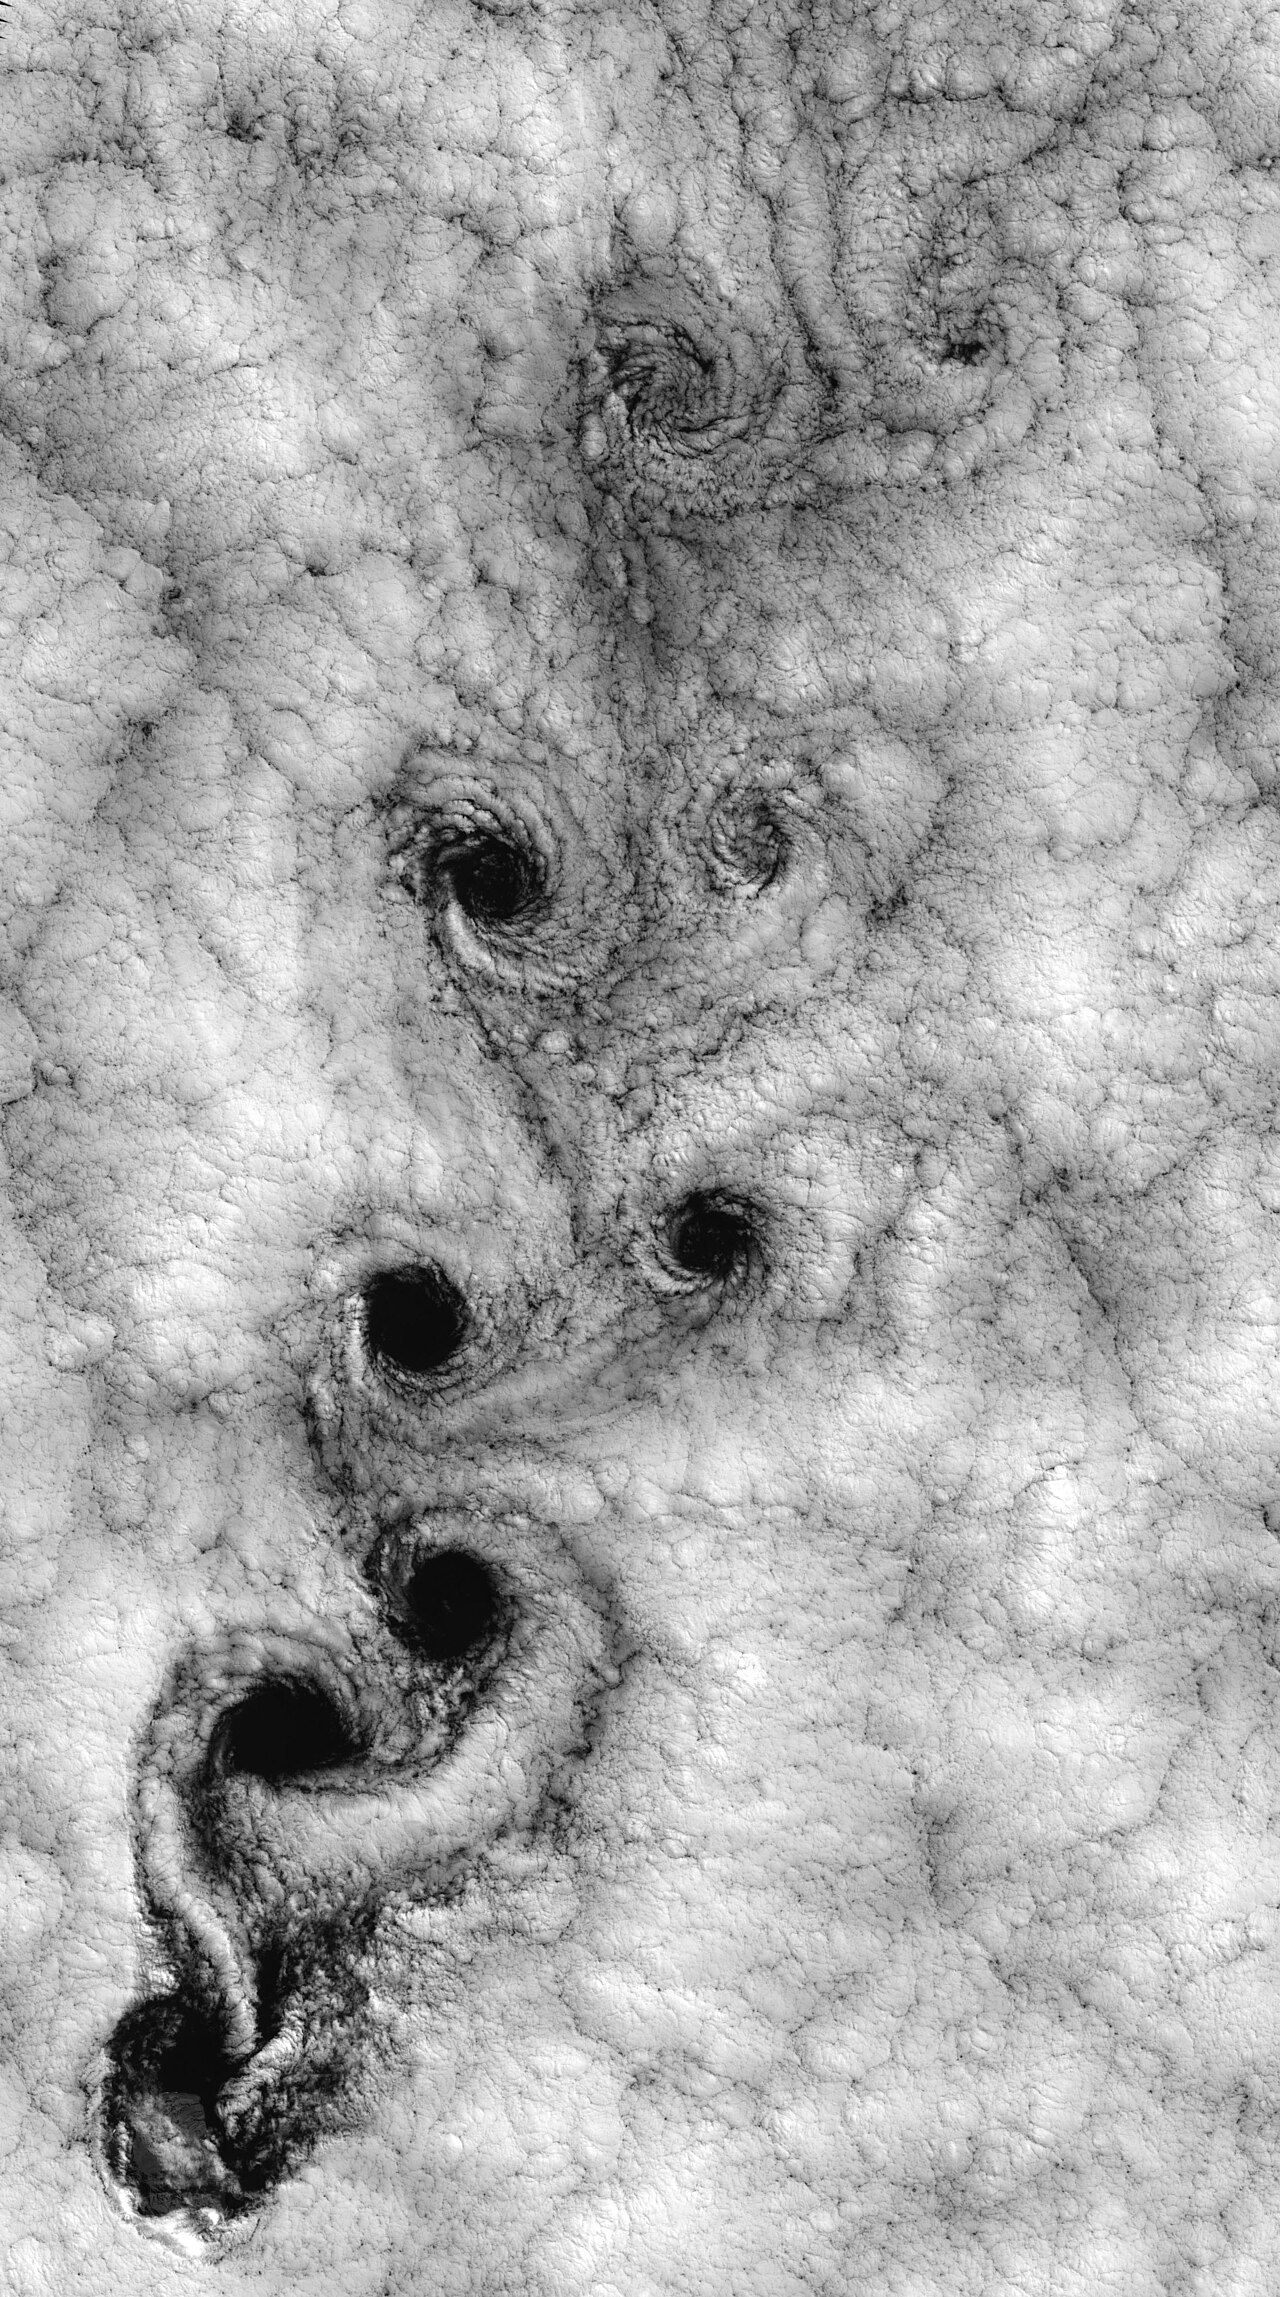
\includegraphics[width=0.34\linewidth]{images/book4/karman-vortex-street.jpg}

{\small شارع دوامات فون كارمان في الغيوم في مصبّ جزيرة، منظورًا من الفضاء: ذيل أسطوانة عند \omterm{def:b2:viscous-flows:reynolds}{عدد رينولدز} بضع مئات، مرسومًا على مقياس مئة كيلومتر (ناسا).}
\end{omfigure}

\section{مسألة: الدم والنفط الخام والمطر}

\begin{problem}[{مسألة نهاية الأسبوع --- القوانين اللزجة نفسها في
شريان، وفي خط أنابيب طوله ألف كيلومتر، وفي قطرة ساقطة}]
\label{pb:b2:viscous-flows:1}

\medskip
\noindent\textbf{الجزء I --- الدم.}
الدم: $\rho = \qty{1060}{kg/m^3}$، و $\eta = \qty{3.5e-3}{Pa.s}$ (معامَلًا
مائعًا نيوتنيًّا)؛ والدفق القلبي $D_V = \qty{5.0}{L/min}$.
\begin{enumerate}
  \item الأبهر، ونصف قطره \qty{1.25}{cm}: السرعة الوسطى \omterm{def:b2:viscous-flows:reynolds}{وعدد
        رينولدز} والنظام.
  \item ولو كان الجريان في الأبهر \omterm{prop:b2:viscous-flows:poiseuille}{جريان بوازوي}، فما السرعة
        العظمى \omterm{def:b2:viscous-flows:viscosity}{وإجهاد القصّ} عند الجدار؟ (فالبطانة الغشائية
        تستشعر إجهادات رتبتها \qty{1}{Pa}.)
  \item وشعيرة نصف قطرها \qty{4.0}{\micro m} تحمل الدم بالسرعة
        \qty{0.30}{mm/s}: أوجد \omterm{def:b2:viscous-flows:reynolds}{عدد رينولدز}؛ وانخفاض الضغط على
        طولها \qty{1.0}{mm}، بالباسكال وبميليمترات الزئبق
        (و \qty{1}{mmHg} تساوي \qty{133}{Pa}).
  \item الزمن الذي تستغرقه كرية حمراء في عبور الشعيرة؛ ولماذا
        تكون هذه هي الرتبة الصحيحة لتبادل الغازات؟
  \item الشرينات (نصف قطرها \qty{10}{\micro m}، وطولها \qty{2.0}{mm}، وعددها $10^8$
        على التوازي): أوجد مقاومة المجموعة وانخفاض الضغط
        عبرها عند الدفق القلبي الكامل.
  \item والانخفاض الكلي من الشرايين إلى الأوردة \qty{13}{kPa}: أوجد
        الاستطاعة الميكانيكية التي يقدّمها البطين الأيسر. وقارنها
        بجسم استطاعته \qty{100}{W}.
  \item ويخفض تضيّق نصف قطر شريان إكليلي بنسبة $40\%$
        على طول قصير: بأي معامل ترتفع مقاومته؛ ولماذا قد تبقى
        عضلة القلب في المصبّ مرويّة في الراحة لا في الجهد.
  \item وأثناء جهد شديد يبلغ الدفق القلبي \qty{25}{L/min}:
        فما \omterm{def:b2:viscous-flows:reynolds}{عدد رينولدز} في الأبهر، وما النظام؟
  \item والدم ليس نيوتنيًّا: إذ تهبط لزوجته الظاهرية عند معدل
        القصّ الكبير وترتفع عند الصغير. فأي الأوعية السابقة
        أشدّ تأثرًا، وفي أي اتجاه؟
\end{enumerate}

\medskip
\noindent\textbf{الجزء II --- خط الأنابيب.}
خط أنابيب نفط خام: قطره $D = \qty{1.2}{m}$، وطوله $L = \qty{1300}{km}$،
وتدفقه $D_V = \qty{3.0}{m^3/s}$؛ والنفط $\rho = \qty{850}{kg/m^3}$، و $\eta =
\qty{2.0e-2}{Pa.s}$ حين يُبقى دافئًا. والاحتكاك المضطرب: $\Delta P = \lambda
(L/D)\tfrac12\rho\langle v\rangle^2$، مع $\lambda = 0.316/\mathrm{Re}^{1/4}$.
\begin{enumerate}[resume]
  \item السرعة الوسطى \omterm{def:b2:viscous-flows:reynolds}{وعدد رينولدز}؛ والنظام.
  \item انخفاض الضغط في الكيلومتر وعلى الخط كله.
  \item ويتحمل الأنبوب \qty{80}{bar}: فما أصغر عدد لمحطات الضخّ
        على امتداد الخط؟
  \item الاستطاعة الكلية للضخّ؛ والطاقة في المتر المكعب من
        النفط المسلَّم، مقارنةً بمحتوى النفط من الطاقة (\qty{36}{GJ/m^3}).
  \item وأي انخفاض يتنبأ به قانون بوازوي؟ علّق على كلفة
        الاضطراب (وعلى سبب حقن مضافات بوليمرية تؤخّر
        الاضطراب في بعض خطوط الأنابيب).
  \item وفي الشتاء يبلغ النفط غير المسخَّن $\eta = \qty{2.0}{Pa.s}$:
        فما \omterm{def:b2:viscous-flows:reynolds}{عدد رينولدز} الجديد والنظام؛ وما انخفاض الضغط على الخط
        بالقانون الملائم؟ وما نتيجة ذلك للتصميم (فالخط الحقيقي
        معزول والنفط يُبقى دافئًا)؟
  \item زمن عبور النفط من طرف إلى آخر.
  \item \omterm{def:b2:viscous-flows:viscosity}{إجهاد القصّ} عند الجدار في الحالة الدافئة المضطربة،
        انطلاقًا من انخفاض الضغط؛ \omterm{def:b2:rigid-body-mechanics:contact}{وقوة الاحتكاك} الكلية على جدار الأنبوب.
  \item والتدفق نفسه في أنبوب قطره \qty{1.0}{m}: بأي معامل يتغير
        انخفاض الضغط المضطرب؟
  \item وتُحمَل حبة رمل قطرها \qty{0.10}{mm} ($\rho_s = \qty{2650}{kg/m^3}$)
        في النفط الدافئ: أوجد سرعة ترسيب ستوكس، \omterm{def:b2:viscous-flows:reynolds}{وعدد رينولدز}
        للحبة، وزمن الترسيب عبر الأنبوب. وقارن بتقلبات السرعة
        المضطربة، وهي بضعة بالمئة من $\langle v
        \rangle$: أيترسّب الرمل في خط الأنابيب العامل؟ وفي
        الخط المتوقف؟
\end{enumerate}

\medskip
\noindent\textbf{الجزء III --- القطرات.}
الهواء: $\rho = \qty{1.2}{kg/m^3}$، و $\eta = \qty{1.8e-5}{Pa.s}$؛ والماء $\rho_w =
\qty{1000}{kg/m^3}$، و $\gamma = \qty{0.072}{N/m}$.
\begin{enumerate}[resume]
  \item قطرة غيم قطرها \qty{10}{\micro m}: أوجد سرعة ستوكس الحدّية،
        \omterm{def:b2:viscous-flows:reynolds}{وعدد رينولدز}، وزمن السقوط \qty{1}{km}؛ ولماذا يبقى الغيم.
  \item رذاذ قطره \qty{0.20}{mm}: سرعة ستوكس \omterm{def:b2:viscous-flows:reynolds}{وعدد رينولدز}؛ أيبقى
        ستوكس موثوقًا؟
  \item قطرة مطر قطرها \qty{2.0}{mm}: بيّن أن ستوكس يخفق، وأوجد
        \omterm{prop:b2:viscous-flows:stokes}{السرعة الحدّية} مع $C_x = 0.5$. وزمن السقوط من \qty{1}{km}.
  \item وفي تيار صاعد سرعته \qty{1}{cm/s}، أترتفع قطرة الغيم أم
        تسقط؟ وأي تيار صاعد يحمل قطرة الرذاذ؟
  \item \omterm{rem:b2:viscous-flows:capillarity}{ضغط لابلاس} داخل القطرات الثلاث؛ وقارنه \omterm{thm:b2:euler-bernoulli:bernoulli}{بالضغط
        الديناميكي} $\tfrac12\rho v_\infty^2$ لكل منها، واشرح لماذا
        تتفلطح قطرات المطر الكبيرة وتتفكك فوق نحو \qty{5}{mm}.
  \item أعطِ في جدول واحد، لجريانات هذه المسألة الثمانية، \omterm{def:b2:viscous-flows:reynolds}{عدد
        رينولدز} والقانون الذي يحكمه.
\end{enumerate}
\end{problem}
